\chapter{Практическая часть}


В листинге 3.1 представлена реализация системы массового обслуживания на языке имитационного моделирования GPSS

\begin{lstlisting}[caption=Реализация системы массового обслуживания]
GENERATE (UNIFORM(1, 1.0, 10.0))
IN QUEUE RequestQueue
SEIZE Service
DEPART RequestQueue
ADVANCE (POISSON(1, 1))
RELEASE Service
TRANSFER 0.7,OUT,IN
OUT TERMINATE 0
GENERATE 100000
TERMINATE 1
START 1
\end{lstlisting}

\clearpage

На рисунке~\ref{plt:gpss_res} демонстрируется работа программы. Максимальная длина очереди при вероятности возврата заявки 70\% равна 10 заявок.

\begin{figure}[h]
	\centering
	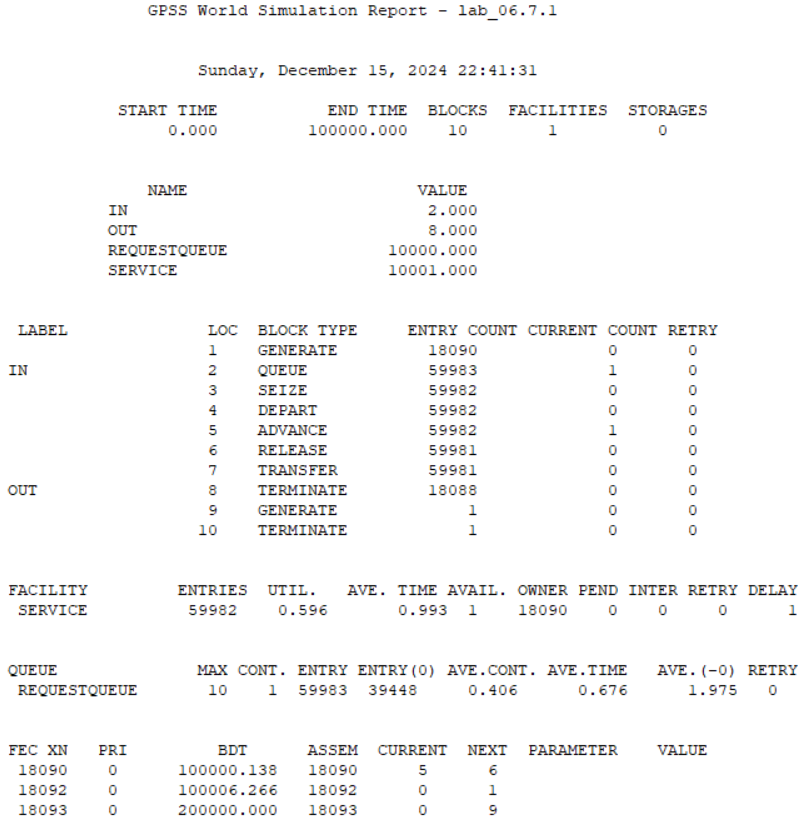
\includegraphics[height=0.55\textheight]{img/gpss_res.png}
	\caption{Отчёт системы массового обслуживания}
	\label{plt:gpss_res}
\end{figure}

